\chapter{Foundations}
This project is fundamentally about combining existing technologies. In particular, the two most important ones are MicroPsi 2, the most ambitious framework aiming to implement the ideas of the Psi theory, and Minecraft, the super-popular sandbox-videogame.

To understand how and why they were chosen, a brief history of their creation as well as explanations of their basic ideas and relevant insights to their architecture are what this chapter is about.

    \section{Psi Implementations}
Psi has been implemented by different groups at different times. The first implementations are by Dörner and his associates themselves~(see figure \ref{psi_screen}). They used Pascal and developed it for windows environments. This implementation can still be downloaded and runs on Windows 7 installations, for example.

\begin{figure}[h]
  \centering
    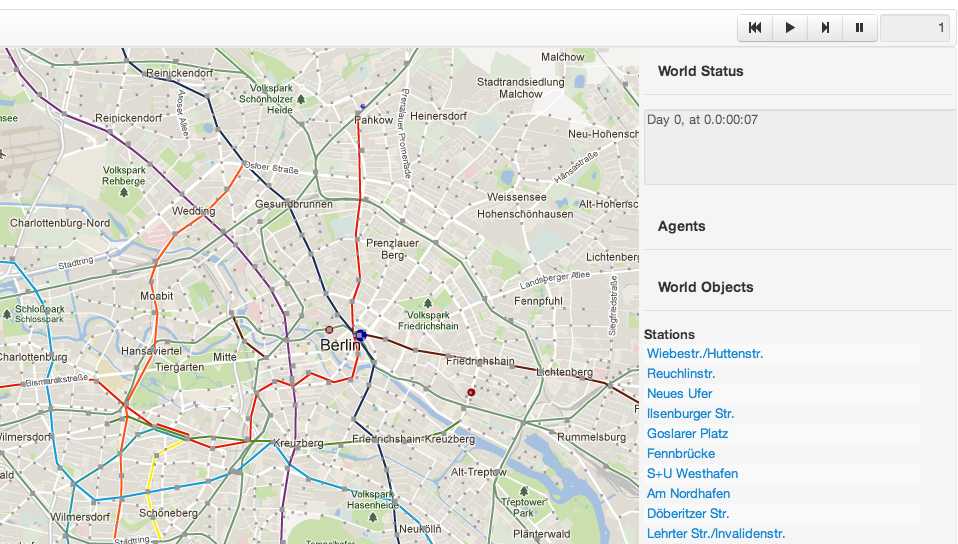
\includegraphics[width=10cm]{graphics/mp2_berlin}
  \caption{MicroPsi simulation environment Berlin}
  \label{mp2_berlin}
\end{figure}

The work on Dörner's team's implementation has not been continued, so Joscha Bach and his associates built new implementations of Psi.

From 2003 to 2009 they built an implementation in Java as a set of plugins for the Eclipse IDE called MicroPsi. It included of a graphical editor and a 3D simulation-environment. Aiming at better understandability and to maintain platform independence, MicroPsi has been built ground up again in 2012 --- using more lightweight Python code. What is remarkable about the new implementation called MicroPsi 2 (in the following MicroPsi), is that the simulation is deployed as a web application and the graphical interface is completely rendered inside a webbrowser --- using state-of-the-art internet- and webapplication-technologies. It is based upon HTML as well as Javascript and the communication in between the browser and the simulation is managed via JSON remote procedure calls. Many GUI components of Twitter's Bootstrap library as well as the JavaScript graphics library PaperJS are used.~\cite{conf/agi/Bach12}

According to the concepts of the Psi Theory, MicroPsi simulates agents as neuro-symbolic spreading activation networks. Agents can be placed and researched in simulation environments or physically embodied as robots.~\cite{conf/agi/Bach12}
        
Even though there have been more complex simulation environments (e.g. 3D-worlds) for previous implementations of Psi-architectures, the relatively new version of MicroPsi has only two fairly simple ones: a 2D-Island and a map of the public transportation system of Berlin~(see figure~\ref{mp2_berlin}). Instead of building another 3D-world, with this project we set out for something more experimental.

\begin{figure}[h]
  \centering
    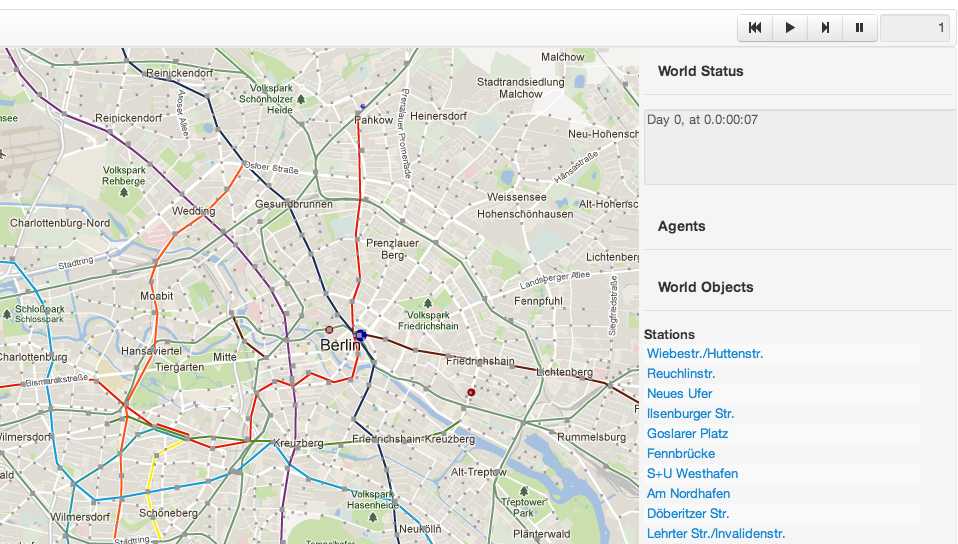
\includegraphics[width=10cm]{graphics/mp2_berlin}
  \caption{MicroPsi simulation environment Berlin}
  \label{mp2_berlin}
\end{figure}

        \section{MicroPsi 2 Module Overview}
MicroPsi's modular structure is fairly easy to understand~(see figure ~\ref{micropsi2_modules}). At first, one can differentiate between the server component (or the web-interface) and the actual simulation code (called "core").

In a minimal setup MicroPsi runs three threads. One thread for the webserver, one for the world simulation and one for every world-adapter (or agent). If more then one agent or more than one world are launched, they are instantiated as additional threads.

Furthermore, the core consists of a runtime component, a user and a configuration manager. The runtime works independently of the server and can also by deployed for commandline interaction or other GUIs. It manages the simulations worlds as well as the agents (node net embodiments) and the world-adapters.~\cite{conf/agi/Bach12}
\\          
          
\begin{figure}[h]
  \centering
    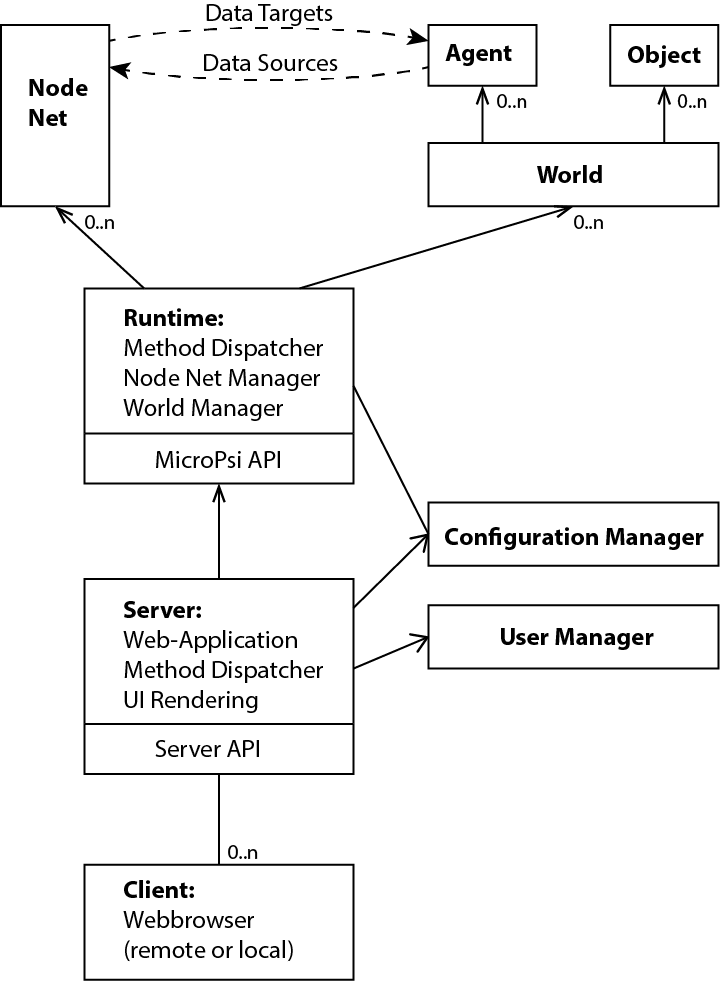
\includegraphics[width=10cm]{graphics/micropsi2_uml}
  \caption{The MicroPsi 2 architecture~\cite{conf/agi/Bach12}}
  \label{micropsi2_modules}
\end{figure}
            
        \paragraph{Agents}
MicroPsi defines agents as node nets or, to be more specific, hierarchical spreading activation networks. They are an "abstraction of the information processing provided by brains"~\cite{conf/agi/Bach12}. The assigned world-adapter provides data sources and data targets to manage the communication in between the node net and the simulation environment. They represent the agent's sensory input and motoric output. Sophisticated interconnection of those enables interaction with the environment.~\cite{conf/agi/Bach12}
       
        \paragraph{Worlds}
The simulations worlds are the environments in which we can study our agent's behavior. Worlds need to provide a worldadapter --- the interface in between a node net and the simulation. Data sources and data targets have to be defined carefully, to get a functional and meaningful experiment going. Node nets and environments may be updated asynchronously.~\cite{conf/agi/Bach12}

The kind of data the world adapter interfaces, is not specified any further, which gives developers the opportunity to experiment with classic simulation worlds as well as exotic applications (eg. stock data). At the time of the development of the original development of the framework, the priorized application was building a framework for knowledge representation.~\cite{conf/agi/Bach12}

    \section{Minecraft}
The story of Minecraft has many interesting aspects, but first and foremost it is a story of immense, unexpected success.

When Markus (``Notch'') Persson built and released the first public version of Minecraft, it soon became clear that his creation resonated with many people. The simple concept of a world entirely build of standard sized building blocks, which the player can create, destroy and relocate one-by-one, enabled many gamers to employ their creativity, explore the Minecraft world and test out it's possibilities and boundaries.

The game has attracted great attention ever since its first release in 2009. Since copies of the game could be obtained commercially for the first time, different versions of the game sold more than 26 million times --- with the PC version priced at about 20 Euros, for example. It should be noted, that Minecraft's development studio Mojang is a so called "indie game developer", that is not associated with any classical game publisher, but distributes copies of their game exclusively via their own website.

Although the game can be downloaded and played as a single packet of software, many scenarios of playing the game consist of running a Minecraft server software, as well as one copy of the client software for each player. It is possible to mimic the official client by implementing the reverse-engineered Client-Server-Protocol and therefore build artificial players that way.

Minecraft is a complex, yet easily accessible virtual world. It is in constant development and new features are added regularly. It has a massive fanbase and a huge community around all kinds of game-modifications.

Another interesting aspect about Minecraft is the procedural semantic the game world is generated with. Trees in Minecraft, for example, may share a similar structure that consists of a trunk and leave-covered branches spreading out fractally, but the particular characteristics of each tree are generated randomly. This makes a Minecraft world somewhat more realistic than many other videogames.

        \subsection{What is a Minecraft world?}
In this section basic concepts of the game are described (in regards to our A.I. interface). Minecraft worlds are build out of blocks~(see figure ~\ref{mc_block}). Blocks are cubes. There are different types (materials) of blocks and they share a single size, which converts to the basic distance unit of Minecraft. One unit can be thought of as roughly equaling one meter.

\begin{figure}[h]
  \centering
    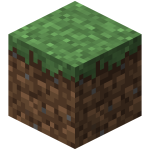
\includegraphics[width=1cm]{graphics/block}
  \caption{A "grass" Minecraft Block (CC-BY-3.0 Mojang AB)\cite{image_mob}}
  \label{mc_block}
\end{figure}
        
A chunk~(see figure ~\ref{mc_chunk}) is a segment of the Minecraft world that is 16 blocks long, 16 blocks wide and 256 blocks high (or deep) and therefore consists of up to 65,536 blocks.~\cite{mcwiki_chunks}

\begin{figure}[h]
  \centering
    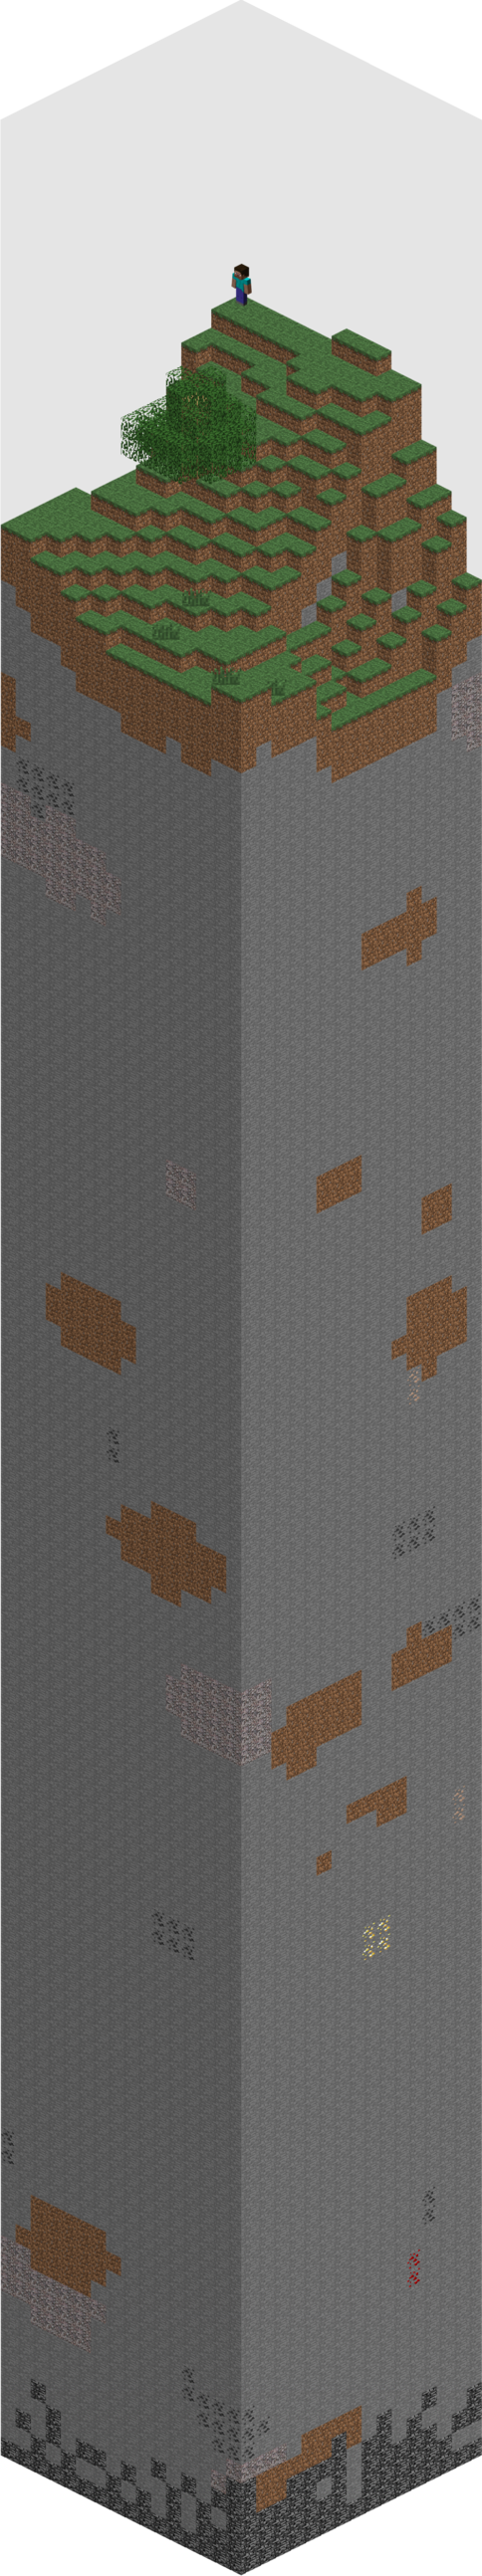
\includegraphics[width=1cm]{graphics/chunk}
  \caption{A Chunk (CC-BY-3.0 Mojang AB)\cite{image_mob}}
  \label{mc_chunk}
\end{figure}

"The player"~(see figure ~\ref{mc_player}) is what the playable game-character in Minecraft is called. It is usually displayed humanoid.

\begin{figure}[h]
  \centering
    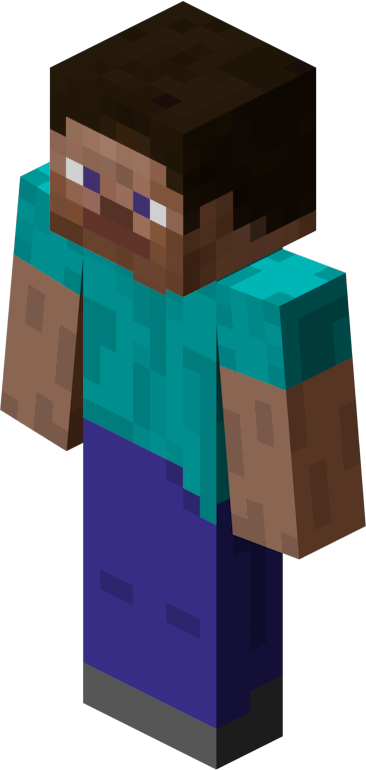
\includegraphics[width=1cm]{graphics/player}
  \caption{"the player" (CC-BY-3.0 Mojang AB)\cite{image_mob}}
  \label{mc_player}
\end{figure}

Also, a Minecraft world has a day-night-cycle with 24 Minecraft hours converting to 14 minutes by default

The game itself has no predefined goals. Players can walk around, discover the generated world (see figure \ref{mc_mechanics} 1) and collect resources by ``destroying'' blocks , with the generated resources equaling the block type. They can combine different resources to ``craft'' items. For example, a player can destroy the blocks that represent a tree (2). The gained ``wood'' ressource could then be used to craft a wooden pickaxe, which could then be used to dig into the ground more effectively to ``mine'' more rare resources, like iron or gold.

\begin{figure}[h]
  \centering
    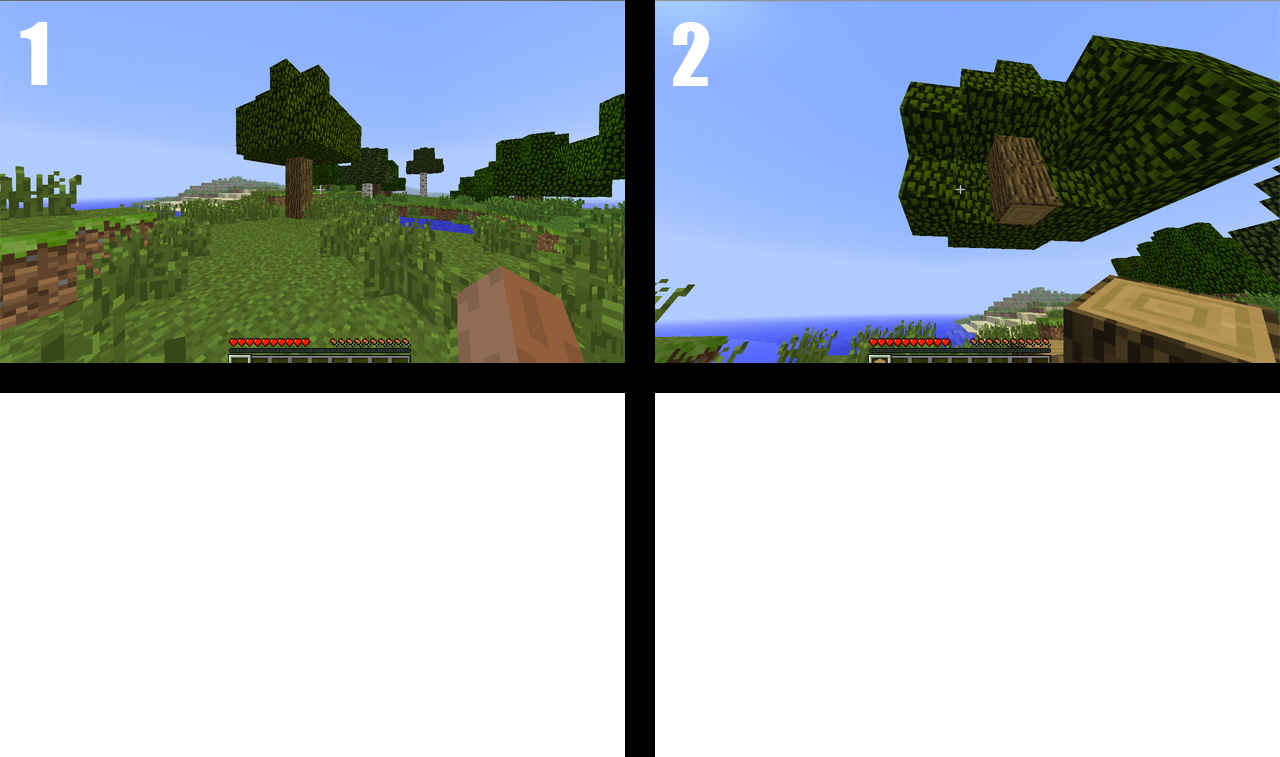
\includegraphics[width=15cm]{graphics/minecraft_mechanics}
  \caption{Minecraft Basic Mechanics  (CC-BY-3.0 Mojang AB)} %TODO find out copyright
  \label{mc_mechanics}
\end{figure}

There exist different game modes. The original "survival" mode adds monsters that attack the player at night. What solutions to survive the player comes up with (eg. building shelter or fighting the monsters) is left up to him or her.

In "creative" mode, the player is not beeing attacked by monsters, has the ability to fly and instant access to unlimited ressources.

The mode of a Minecraft world does not effect the functionality of this project.

        \subsection{The Client Server Protocol}
Minecrafts Client-Server-Protocol is not publicly documented by the developers themselves. However, the modding-community gathered full knowledge and understanding of its structure (probably by using reverse engineering techniques). The protocol is based on packets. 

Packets are either "server to client", "client to server" or "Two-Way" and begin with a "Packet ID" byte. The structure of the packet's payload depends on it's Packet ID.
 
To give an example of one of the easier packets, the "Client Position"-Packet is fairly straight-forward~(see figure \ref{mc_packet}). It is exclusively send from clients to servers and starts with it's Packet ID (as every packet does), followed by the X- and Y-coordinates as doubles, the stance value as a double, which is used to to modify the players bounding box, another double for the Z-coordinate and eventually a boolean that describes if the player is on the ground or not.~\cite{protocol}

\begin{table}[htb]
\centering
\begin{tabular}{|c|c|c|}\hline

    Field Name & Field Type & Notes \\ \hline
   Packet ID & Byte & 0x0B \\ \hline
   X & double & Absolute position \\ \hline
   Y & double & Absolute position \\ \hline
   Stance & double & Used to modify the players bounding box \\ \hline
   Z & double & Absolute position \\ \hline
   On Ground & boolean & Derived from packet 0x0A \\ \hline
   
\end{tabular}
\caption{Structure of the packet ``Player Position (0x0B)''~\cite{protocol}}
\label{mc_packet}
\end{table}

Knowledge of this datastructure is already sufficient to move around in the Minecraft world. To go forward, one has to figure out the players current position, calculate the absolute coordinates of the destination of the movement in regard of it and send a Client Position packet with these coordinates to the server. If the destination is not more than 100 blocks away from the origin of the movement, the server accepts the packet. In the official Minecraft client, a players movement from one point to the other is rendered with a walking animation.

Other than movement, packet structures are defined for every aspect of the game. May it be the initial handshake, the creation or destruction of blocks or activities of other player- or non-player-characters.

This protocol is what a custom Minecraft client needs to speak.

        \subsection{Suitability of Minecraft as a simulation environment}
There are a number of reasons why using Minecraft as a simulation environment could be useful and lead to interesting results.

First, the game itself is easily accessible. It is developed using Java (for both the client and the server software) and therefore up to a certain extend platform independent. The "desktop computer version" is being sold for Windows, Mac OS X and Linux devices. There are official ports for Android, iOS, Xbox 360, the Raspberry Pi an a version for the upcoming game console "Xbox One" is announced. The desktop versions are priced at 19.95 euros, which makes it affordable to a large audience.
%TODO find out how to typeset €

The game itself already has an enormous fanbase. It is (like most videogames) especially popular among teenagers. Minecraft being loved by so many people could benefit this project, in terms of leading to increased attention.

The game's developer has proven many times that it acts generously towards  other developers, when it comes to the creation of game modifications and content that uses, or changes original Minecraft intellectual property. In other words: Mojang is not restrictive towards users doing all kinds of things with their creations. This led to the availability of a fairly complete community-sourced  documentation and explanation of virtually every aspect of the game --- including it's software architecture, data structure and protocols. This is useful for this project, as chances are low that they will have anything against using Minecraft for this project in the foreseeable future. %(In fact, the game's A.I. creator Jon Kagström seems to be fond of this project)

The Minecraft world with it's logic, semantic and functionalities offers possibilities for an A.I. to proove being able to interact with the environment --- in primitive ways (e.g. moving around), as well as with increasingly complex tasks like building, collecting resources, crafting items and interacting appropriately with both well-disposed and hostile other entities.

The semantics of the gameworld share characteristics with the real world. Moving through a Minecraft environment, one quickly realizes that the game has generated different biomes (eg. forest or tundra). Also, trees, rivers, mountains and ore veins are neither hard-coded, nor appear completely randomly, but are generated procedurally and their structure appears to be (somewhat) fractal.
        
Using Minecraft as a simulation environment will give Psi agents possibilities to show off, what kind of sophisticated behavior it is capable of.

    \section{Minecraft Bots}
There exist many projects , that could be considered Minecraft ``bots''. One has to differentiate in between two types. On the one hand there are those, that mimic an entire client software and facilitate communication with the server on the default client software's behalf. On the other hand there are bots which are modifications of the original client (or server) software and usually add non player characters --- like animals and other non-human creatures --- to the game. The code is usually injected through one of the popular ``modloaders'' (eg. Minecraft Forge).

One example (and probably the most advanced one) for an entire bot framework that replaces the client is Mineflayer.~\cite{github_mineflayer} It has a high-level abstraction of the environment (eg. entity knowledge and tracking) and is written in JavaScript using node.js. However, it has not been used for this project, because a python implementation was aimed for.

Opposed to Mineflayer, an example for ``game modification'' bots are the ``Cubebots'' --- fan-made non-player characters that aim to help Minecraft players with mundane tasks.\cite{mcforums_cubebots}

    \subsection{Spock by Nick Gamberini}
Developed by Nick Gamberini, spock is an open-source bot framework (and as such also a Minecraft client) written in Python. It has been chosen to become an essential part of this project for two reasons: being written in Python it painlessly integrates in the existing MicroPsi code and the absence of dependencies (with one exception) leave the code understandable and easy to deploy.
    
    \subsection{Protocol Implementation in Spock}
The Minecraft protocol implementation in spock is straight-forward~(see figure\ref{snippet_structures}). The necessary data structures are stored seperately and can be accessed globally.

		
		\begin{figure}[ht]
			\centering
			\begin{minipage}{11cm}
				\begin{pseudocode}
names = {
	0x00: "Keep Alive",
	0x01: "Login Request",
	0x02: "Handshake",
	0x03: "Chat Message",
	...

structs = {
	#Keep-alive
	0x00: ("int", "value"),
	#Login request
	0x01: (
			("int", "entity_id"),
			("string", "level_type"),
			("byte", "game_mode"),
			("byte", "dimension"),
			("byte", "difficulty"),
			("byte", "not_used"),
			("ubyte", "max_players")),
	...
					\end{pseudocode}
				\caption{data structures for the packet IDs and structures}
				\label{snippet_structures}
			\end{minipage}
		\end{figure}
		
The structures are used to parse each packet apropriately~(see figure \ref{snippet_parse}).

		\begin{figure}[ht]
			\centering
			\begin{minipage}{11cm}
				\begin{pseudocode}
	def decode(self, bbuff):
		#Ident
		self.ident = datautils.unpack(bbuff, 'ubyte')
		
		#print hex(self.ident)
		
		#Payload
		for dtype, name in mcdata.structs[self.ident][self.direction]:
			self.data[name] = datautils.unpack(bbuff, dtype)
					\end{pseudocode}
				\caption{function for decoding packets}
				\label{snippet_parse}
			\end{minipage}
		\end{figure}

\section{Python Multimedia Libraries and Minecraft Clones}
Minecraft's success inspired many other projects - including a number of Minecraft-like games in a wide variety of programming languages and environments.

Interesting projects include Skycraft~\cite{skycraft}, a Minecraft-like browser-game based on WebGL.

A particular project, that has the same name as the original game that inspired it, is ``Minecraft'' by Michael Fogleman. It is a simple Minecraft clone in under 600 lines of Python and gained some popularity on reddit~\cite{fogle-reddit} and Hacker News.~\cite{fogle_hn}

It is comparably easy to understand and modify and has been used for the visualization component of this project. It is based on the Python multimedia library pyglet~\cite{pyglet}.

